\newpage
\section{TGGs in action}
\genHeader
\label{sect:TGGs_in_Action}

In order to perform a forwards or backwards transformation, we need to actually create something for the TGG to work with. In other words, we need to create an
instance model\footnote{For a detailed review of instances and how to create them, refer to Part II, Section 3} of either our target or our source metamodel!
Since dictionaries are of a much simpler structure, let's start with the backwards transformation.

\begin{itemize}

\item[$\blacktriangleright$] Navigate to \texttt{Dictionary\-Language/model/} and open \texttt{Dictio\-nary\-Lang\-uage.ecore}. Expand the tree and create a new
dynamic instance of a \texttt{Dictionary} named \texttt{target.xmi}. Don't quickly close the window by pressing \texttt{finish}! Make sure you persist the instance in
\texttt{Learn\-ing\-Box\-To\-Dictionary\-In\-te\-gra\-tion/in\-stan\-ces/} (Fig.~\ref{eclipse:create_instance_dict}).

\begin{figure}[htbp]
\begin{center}
  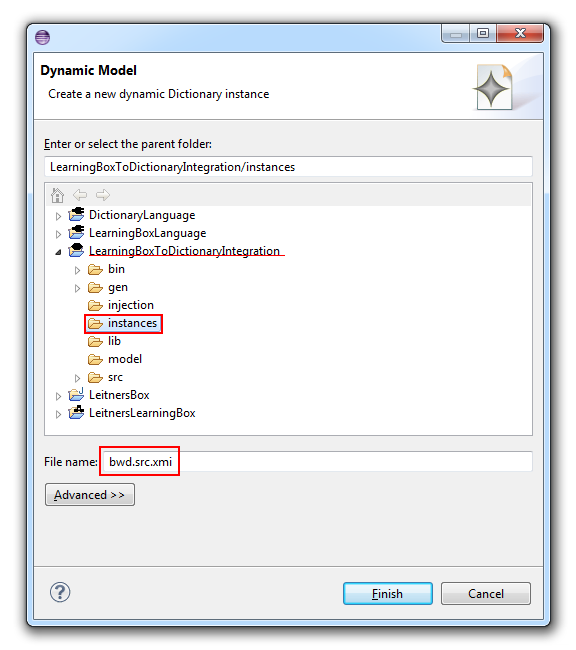
\includegraphics[width=0.8\textwidth]{eclipse_dictionaryInstance}
  \caption{Create a dynamic instance of \texttt{Dictionary}}
  \label{eclipse:create_instance_dict}
\end{center}
\end{figure}

\newpage

\item[$\blacktriangleright$] Open the new file and edit the \texttt{Dictionary} properties by double-clicking and setting \texttt{Title} to \texttt{English
Numbers} in the \texttt{Properties} tab below the window.

\vspace{0.5cm}

\item[$\blacktriangleright$] Create three child \texttt{Entry} objects, giving each one a different difficulty level. Don't forget the syntax we created for
each \texttt{entry.content} in the \texttt{CardToEntryRule} when setting up the constraints! Be sure to set this property as \texttt{<word>:<meaning>}. Your
\texttt{target.xmi} should resemble Fig.~\ref{eclipse:dictionaryxmi}.

\vspace{0.5cm}

\begin{figure}[htbp]
\begin{center}
  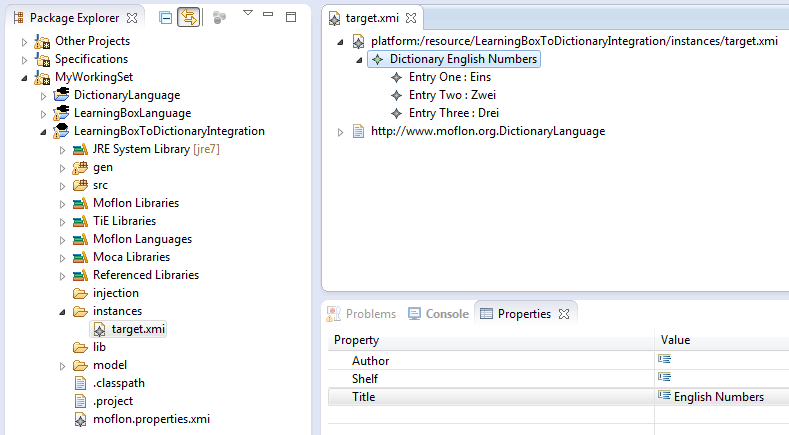
\includegraphics[width=\textwidth]{eclipse_targetThreeEntries}
  \caption{Fill a \texttt{Dictionary} for the transformation}
  \label{eclipse:dictionaryxmi}
\end{center}
\end{figure}

\item[$\blacktriangleright$] Navigate to ``LearningBox\-To\-Dictionary\-In\-te\-gra\-tion\-/src'' and right-click on \texttt{TGGMain.java}. 
\update FIRST INSTANCE: It should resemble BLAH. As you can see, it's the driver to run the complete transformation. Right click the file in the package
exploerer, and Go to ``Run as\ldots/Java Application''

\vspace{0.5cm}

\item[$\blacktriangleright$] Did you get one error message, followed by one success message in eMoflon console window below the editor?
(Fig.~\ref{eclipse:tggERROR}) Perfect! Both of these statements make sense -- our TGG first attempted a forward transformation of \texttt{box} to
\texttt{dictionary} but, given that it was missing the source (\texttt{box}) instance, it was only able to perform a transformation in the backwards direction.

\begin{figure}[htbp]
\begin{center}
  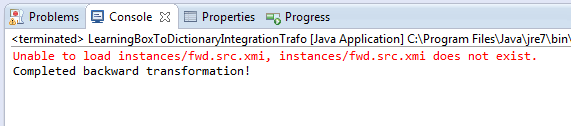
\includegraphics[width=\textwidth]{eclipse_TGGError}
  \caption{A single forward transformation}
  \label{eclipse:tggERROR}
\end{center}
\end{figure}

\newpage

\item[$\blacktriangleright$] Refresh the integration's \texttt{instances} folder. There should now be four new \texttt{.xmi} files. While you created
\texttt{target}, the TGG generated \texttt{corr\_BWD}, the correspondence graph between target and source, \texttt{protocol\_BWD}, a listing of the attempted
steps taken (as well as their results), and \texttt{target.xmi\_BWD}, the output of the transformation. Open this file in the editor.

\item[$\blacktriangleright$] It's a \texttt{Box} of \texttt{English Numbers}! Expand the tree and you'll see our \texttt{Dictionary} in its equivalent
\texttt{Box} format containing three \texttt{Par\-ti\-tions} (Fig.~\ref{eclipse:derivedBOX}). Double click each \texttt{card} and observe how each
\texttt{entry.content} was split into two sides.

\vspace{0.5cm}

\begin{figure}[htbp]
\begin{center}
  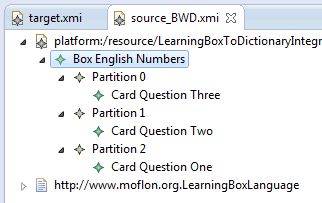
\includegraphics[width=\textwidth]{eclipse_derivedSource}
  \caption{Result of the \emph{backwards} transformation}
  \label{eclipse:derivedBOX}
\end{center}
\end{figure}

\item[$\blacktriangleright$] Congratulations! You have successfully performed your first \emph{backward} transformation from your target model (dictionary) to
your source (Learning box) using TGGs! 

\newpage

\item[$\blacktriangleright$] Don't forget about one of eMoflon's coolest model visualizing features -- the graph viewer.\footnote{Refer to Part 2, Section 4 to
review how to open and use this tool} This is an especially useful tool with TGGs when you need to do a quick confirmation that your transformation was
successful. Drag-and-drop \texttt{Box English Numbers} into the graph view (Fig.~\ref{eclipse:graphView}). You should be able to see each \texttt{Card}'s
container \texttt{partition} and the edges via which they'll move between partitions. 

\vspace{0.5cm}

\begin{figure}[htb]
\begin{center}
  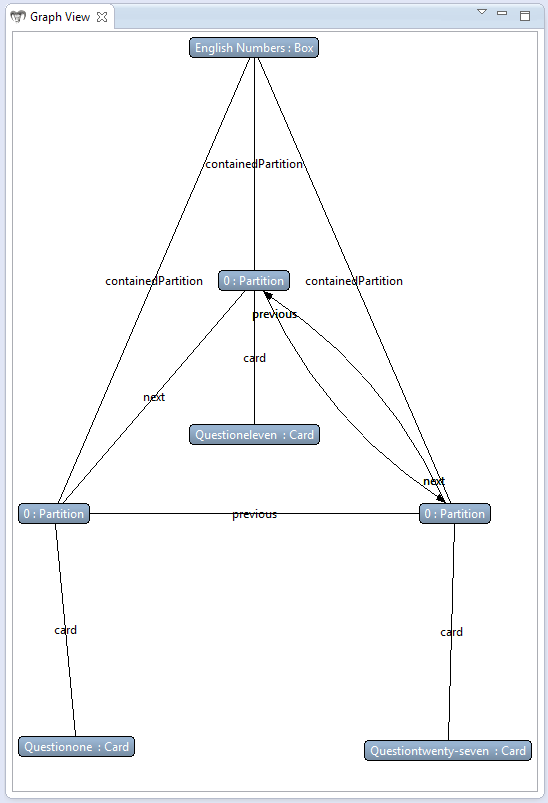
\includegraphics[width=0.6\textwidth]{eclipse_EngNumBoxGraphView}
  \caption{Confirm the transformation with the Graph Viewer}
  \label{eclipse:graphView}
\end{center}
\end{figure}

\vspace{0.5cm}

\item[$\blacktriangleright$] To show that the transformation is actually bidirectional, let's create a source model (thus resolving the error), and run
the TGG again to perform a \emph{forwards} transformation of a \texttt{Box} into a \texttt{Dictionary}. Make a copy of \texttt{target.xmi\_BWD.xmi} and rename
it to \texttt{source.xmi}.

\newpage

\item[$\blacktriangleright$] Run the \texttt{TGGMain.java} again by pressing the green ``Run As\ldots'' icon on the toolbar. You should now have two success
messages in the console window! Refresh the ``instances" folder and compare \texttt{source.xmi\_FWD.xmi} against the original target model. If everything was
created and executed properly, they should look exactly the same. 

\end{itemize}
